This project aims at implementing a MIPS like processor architecture on an FPGA. The MIPS architecture was chosen based on its simplicity and widespread use, which allows the incorporation of ready-made stuff (such as the gcc-compiler) along the way, and compare the results of tests with those of a MIPS simulator.

As special features, forwarding and memory mapped I/O (VGA output and keyboard input) have been implemented. A pong game has also been developed, in order to demonstrate the capabilities of our processor.

\begin{figure}[!h]
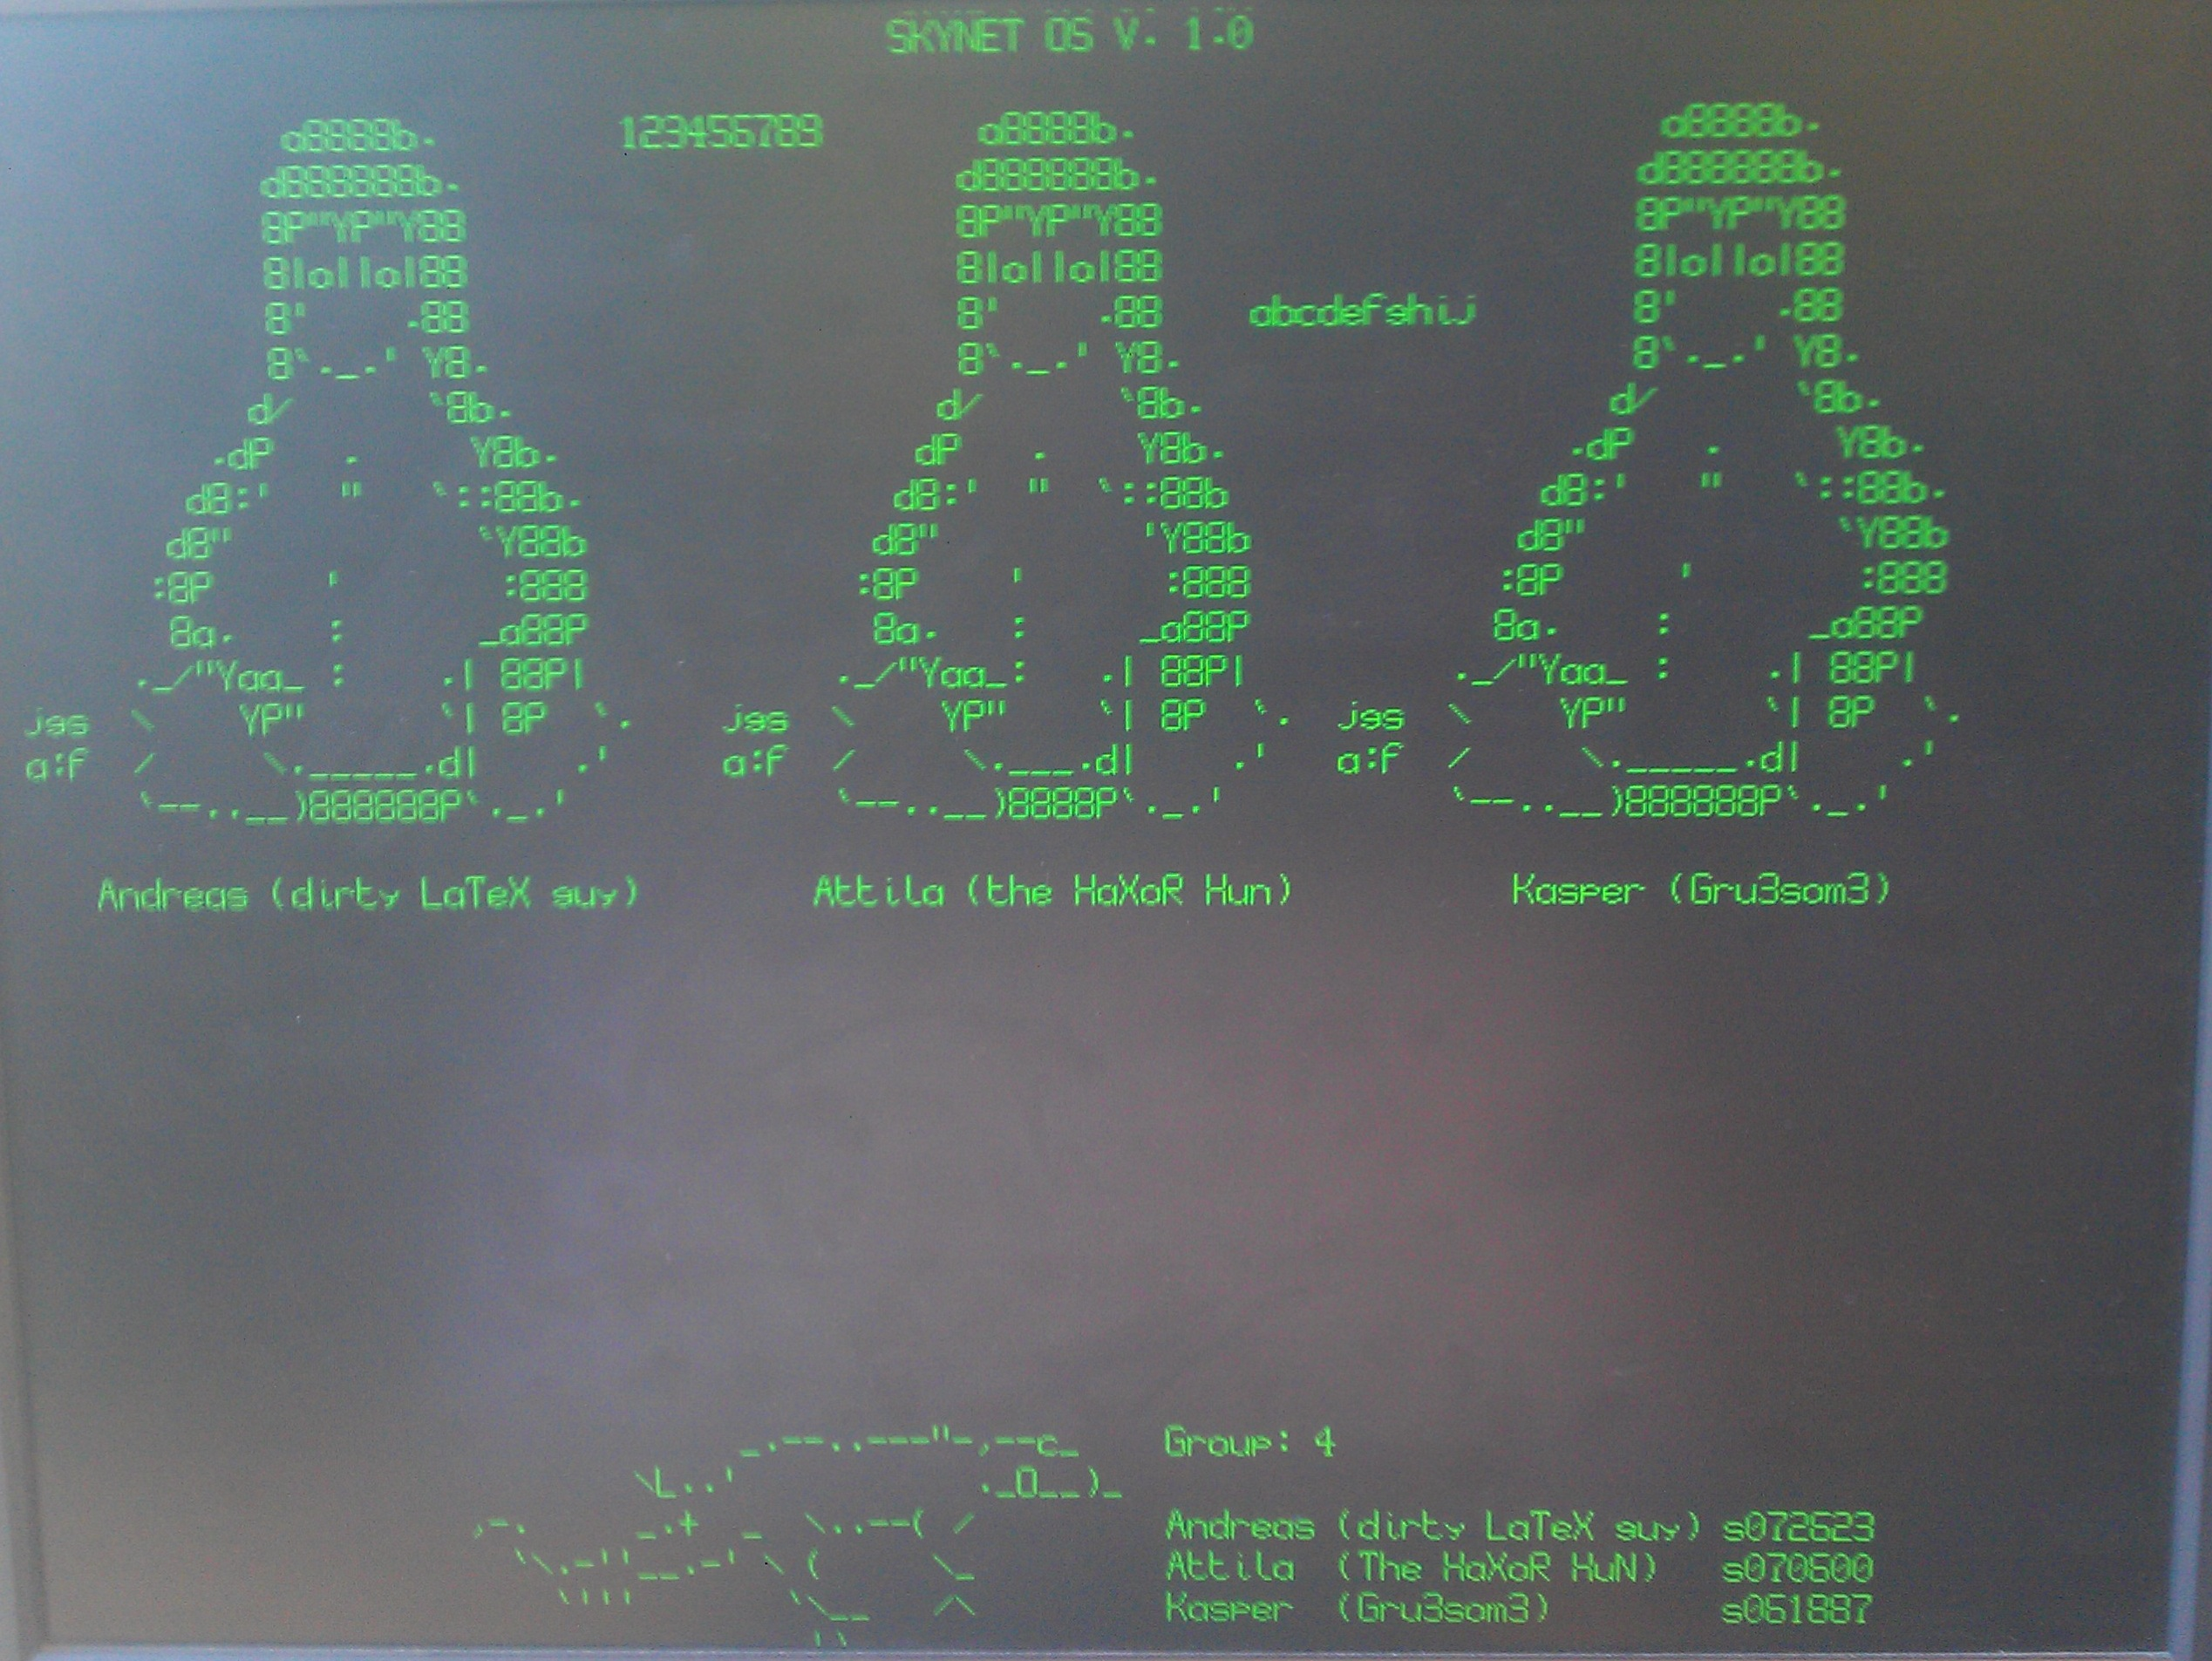
\includegraphics[width=0.45\textwidth]{Images/screen.jpg}
\caption{Splash screen for the pong game.}
\label{fig:splash}
\end{figure}

\paragraph{Outline} After this introductory section, a more thorough introduction to the MIPS architecture and the alternatives to the MIPS is given in section \ref{MIPS}. Section \ref{sec:implementation} deals with the design choices made, and the practical aspects of implementing our MIPS like processor. In section \ref{running} we describe how programs can be compiled and run, and in section \ref{testing} the tests performed are described, along with subsections describing troubles along the way, and relevant suggestions for further improvements in section \ref{sec:future}. Finally, conclusions are drawn in section \ref{conclusion}. The complete list of instructions implemented, along with some relevant code snippets are presented in the Appendix.

\subsection{The MIPS processor}
The MIPS (which is an acronym for Microprocessor without Interlocked Pipeline Stages) processor was first introduced in 1981 by the Company MIPS Technologies. The original MIPS processor was a 32-bit machine, however, newer versions are 64-bit, and it is based on a RISC instruction set architecture (ISA), which simplifies the hardware. The processor implemented in this project, is based on the original 32-bit MIPS.

